\chapter{Implementation and Validation}\makeatletter\def\@currentlabel{Implementation and Validation}\makeatother
\label{chap3}
\lhead{\textbf{CHAPTER 3.} \textit{Implementation and Validation}}


The third chapter details how the \textit{zkpoex} prototype was turned from a design into a working proof-of-concept (PoC). The narrative follows the data as it travels from a local fork of \textsf{geth}, through a purpose-built Rust EVM runner, into the Risc0 zero-knowledge virtual machine and finally back on-chain inside the \texttt{VerifierContract}.  Particular care is paid to the points where an ordinary execution trace is converted into a zero-knowledge receipt so that an external observer can tell, without guessing, that an exploit really exists.

\section{Development Environment}

All components are written in stable Rust 1.86.0 and organised in a multi–crate
workspace stored at \cite{zkpoex}.  The manifest reveals five distinct crates,
each mapped to a well-defined concern:

\begin{lstlisting}[caption={[Workspace Manifest]},language=toml]
[workspace]
resolver = "2"
members  = [
  "shared",        # common utilities and domain types
  "evm-runner",    # pure-Rust EVM interpreter plus spec checker
  "guest",         # code executed inside the zkVM
  "host",          # CLI that drives proving 
  "methods",       # auto-generated Risc0 bindings
]
\end{lstlisting}


\textbf{Why five crates rather than a monolith?}
\begin{itemize}
  \item \textit{shared} is \texttt{no\_std}-friendly and contains only data
        structures, hashing helpers, and logging macros that are reused by every
        other crate.  Isolating it keeps the guest’s dependency tree minimal.
  \item \textit{evm-runner} links the \texttt{evm\,(0.42.0)} interpreter and all
        predicate checking code.  It targets \texttt{std} so that the same
        logic can be fuzz-tested natively before being embedded in the zkVM.
  \item \textit{guest} is compiled for the \texttt{riscv32imac-unknown-none-elf}
        target; splitting it out ensures the guest ELF contains no accidental
        host-only dependencies and gives it a stable \textit{Image ID}.
  \item \textit{host} drives proof generation, serialises inputs, and (optionally)
        pushes the receipt to the on-chain \texttt{VerifierContract}. Keeping
        it separate allows faster incremental builds because it never needs a
        RISC-V cross-compile.
  \item \textit{methods} is produced automatically by \texttt{risc0-build}; it exports the const \texttt{ZKPOEX\_GUEST\_ELF} and the matching \texttt{IMAGE\_ID} is used both by the prover and by verifiers.
\end{itemize}

This breakdown shortens compile times, limits the guest’s code size, and
clarifies the trust boundaries: only \textit{guest} runs in the STARK circuit,
while \textit{host} and \textit{evm-runner} can evolve without forcing a re-audit
of the zero-knowledge core.

\subsection{Toolchain}  

Every machine that builds \textit{zkpoex} uses the exact same Rust compiler and
components.  The file \texttt{rust-toolchain.toml} placed at the workspace
root tells \texttt{rustup} which toolchain to install:

\begin{lstlisting}[caption={[Pinned toolchain]},language=toml]
[toolchain]
channel    = "1.86.0"          # stable compiler known to work
profile    = "minimal"         # std, rustc, cargo only
components = [
  "rustfmt",                   # formatting gate in CI
  "clippy",                    # lints treated as errors
  "rust-src"                   # needed to cross-compile the guest
]
\end{lstlisting}


These are the reasons why this file is important:

\begin{itemize}
  \item Guarantees that the guest ELF, and thus its Risc0 image ID, is reproduced bit-for-bit on every host.
  \item Packages only the pieces required for the project, keeping Docker images small and CI jobs fast.
  \item Adds \texttt{rust-src} so that \texttt{cargo build
        --target x-unknown-none-elf} works out of the box when
        compiling the zkVM guest.
\end{itemize}

With the toolchain pinned, a fresh setup is reduced to three commands:

\begin{lstlisting}[language=bash]
$ rustup toolchain install 1.86.0  # download the pinned compiler
$ rustup default 1.86.0  # active the toolchain
$ cargo build --release  # builds all the crates
$ cargo test             # runs native EVM tests
\end{lstlisting}

No nightly features, external linkers, or patched forks are required with this configuration.


\subsection{Key External Libraries}  

Version 0.1.0 of \textit{zkpoex} (April 2025) relies on only three upstream
crates to generate and validate a proof.  Pinning them at the exact versions
shown below ensures that every audit can rebuild the binary bit-for-bit and
that later ecosystem upgrades cannot silently alter the circuit.

\begin{table}[h]
  \renewcommand{\arraystretch}{1.15}
  \centering
  \begin{tabularx}{\textwidth}{|l|c|X|}
    \hline
    \textbf{Crate} & \textbf{Version} & \textbf{Role in \textit{zkpoex} v0.1.0} \\ \hline
    \texttt{evm}\footnotemark[1]            & 0.42.0 & Canonical byte-for-byte interpreter embedded in the \textit{evm-runner} crate; replays the transaction locally exactly as it would execute on mainnet before the trace enters the zkVM. \\ \hline
    \texttt{risc0\_zkvm}\footnotemark[2]    & 2.0.0  & Supplies the 0STARK prover, guest SDK and Groth16 compression pipeline; every receipt produced by \textit{zkpoex} is ultimately a Risc0 proof. \\ \hline
    \texttt{primitive-types}               & 0.12.0 & Single source of fixed-width Ethereum primitives (\texttt{U256}, \texttt{H160}, \texttt{H256}); guarantees identical encodings on both host and guest. \\ \hline
  \end{tabularx}
  \caption{Pinned library set for the first public release.}
  \label{tbl:libraries}
\end{table}

\footnotetext[1]{Built with the \texttt{with-serde} feature so that full
\texttt{MemoryAccount} objects can be serialised across the host-guest
boundary.}
\footnotetext[2]{Uses the FRI backend shipped by Risc0; the resulting STARK is
compressed to Groth16 for low-gas on-chain verification.}


\textbf{Why no other crates appear here}  
Utilities such as \texttt{serde}, \texttt{tokio}, or \texttt{clap} are secondary crates. They make the CLI convenient but carry no cryptographic weight. Should one of them receive a breaking change, it affects only peripheral code; the core proof remains verifiable so long as the three crates above stay frozen at the versions listed in Table \ref{tbl:libraries}.


\subsection{Auxiliary tooling}  

Foundry is used only to compile the Solidity targets that form the
\ref{case_studies} suite; bytecode and ABI files are committed under the
\texttt{bytecode/} folder so that every reviewer can rebuild the PoC without
installing a global Solidity toolchain.

The day-to-day interface, however, is the \texttt{justfile} shipped in the
repository root.  While it will be deprecated in the next
releases, the current script distils every common workflow compiling contracts,
spinning up a local fork, generating a proof, pushing it on-chain into a single
shell-friendly command.

\begin{itemize}
  \item \textbf{Unit testing} → \texttt{\$ just test-evm} \\
  It compiles the contracts and runs every \texttt{\#[test]} declared in the \textit{evm-runner} crate, proving that each case study really violates its specification at the pure EVM level before any zero-knowledge overhead is added.
  
  \item \textbf{Local proving} → \texttt{\$ just prove}\\
   wraps the entire \textit{host} call in a single command; every argument
      maps one-to-one to a flag in \texttt{host/main.rs}:

      \begin{itemize}
        \item \texttt{function:}   canonical Solidity selector, e.g.\ \texttt{“withdraw(uint256)”}.
        \item \texttt{params:} comma-separated ABI values fed to the selector.
        \item \texttt{context\_state:} path to the JSON file that fixes all accounts and storage slots present \textit{before} the call.
        \item \texttt{program\_spec:} path to the JSON array of post-conditions the guest must try to violate.
        \item \texttt{value:} ETH (in wei) sent along with the call if needed; use \texttt{0} for pure logic bugs if it is not needed.
        \item \texttt{network}   \texttt{local}, \texttt{testnet} (Holesky) or \texttt{mainnet}; selects the RPC endpoint and the canonical Risc0 verifier address.
        \item \texttt{bonsai} (optional, default \texttt{false}) set to \texttt{true} to outsource proving to Bonsai instead of the local GPU.
        \item \texttt{verbose} (optional, default \texttt{false}) enables full \texttt{tracing} output from both host and guest.
      \end{itemize}
  \item \textbf{Bonsai proving:}  
        As told before, adding \texttt{bonsai=true} switches the prover to Risc0’s cloud service.  The script sets \texttt{RISC0\_DEV\_MODE=0} automatically and
        exports the API key from \texttt{BONSAI\_API\_KEY}.
  \item \textbf{On-chain verification:} → \texttt{\$ just onchain-verify } \\
  run the file \texttt{onchain\_verifier.rs} from \textit{host} crate and reads the \allowbreak \texttt{receipt.bin} saved before in the file system after a proof generation, encodes the seal and journal, and submits the Smart-Contract \texttt{verify()} call to the chosen network.
\end{itemize}


Here an example of a single-shot invocation that proves the \texttt{exploit(bool)} bug in the \textit{BasicVulnerable} contract against a local \textsf{anvil} fork:
\begin{lstlisting}[caption={[One-line local proof]},label={example_just},language=bash]
$ just prove "exploit(bool)" true \
    ./shared/examples/basic-vulnerable/context_state.json \
    ./shared/examples/basic-vulnerable/program_spec.json \
    0 local bonsai=false verbose=true
\end{lstlisting}

Please note that within the justfile, it is possible to run the 3 built-in examples with a more streamlined and readable command → \texttt{\$ just example-{name-of-example}-prove}. In Figure \ref{fig:prove_local}, an example of execution from the CLI.

\begin{figure}[h]
  \centering
  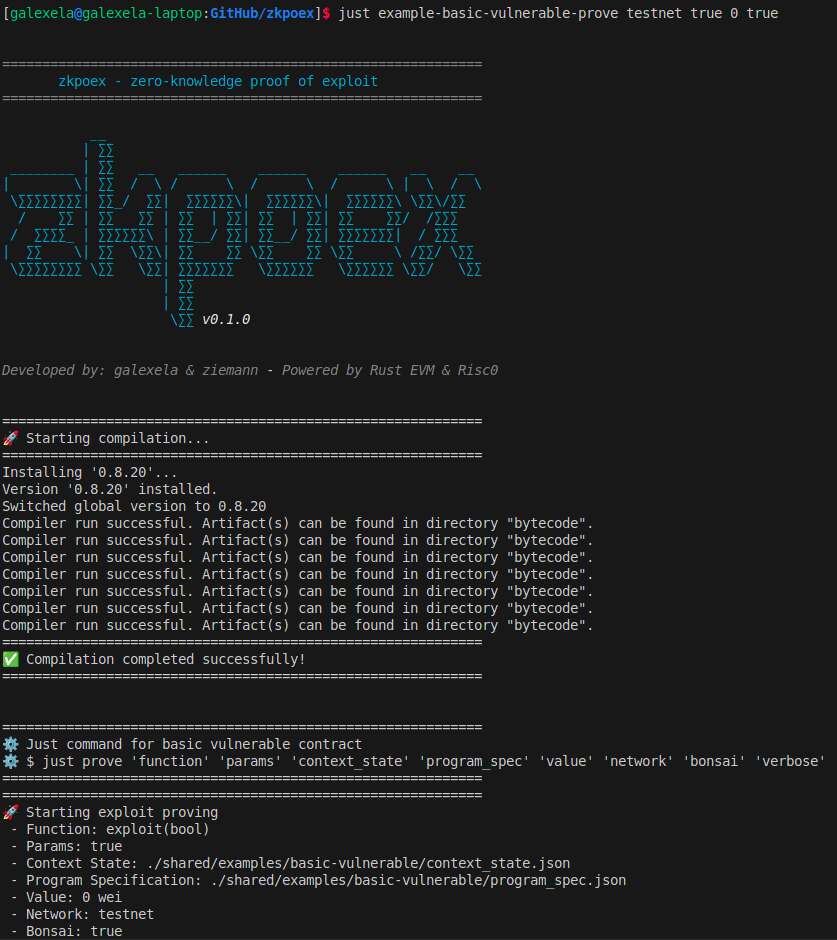
\includegraphics[width=0.8\textwidth]{Images/Chap3/cli_local_proving.png}
  \caption{Terminal output for the \texttt{just prove} recipe.  The script compiles the guest, executes the EVM trace, generates a STARK proof, and finally emits a 304-byte Groth16 receipt ready for on-chain verification.}
  \label{fig:prove_local}
\end{figure}

Newcomers need only skim \texttt{justfile} to discover the available actions. The file keeps all environment variables in one place, validates mandatory secrets (\texttt{WALLET\_PRIV\_KEY}, \texttt{BONSAI\_API\_KEY}) before running, and prints a concise banner with all the logs related to internal script executions to let the user know how the software is running at that time. The \textit{justfile} makes the PoC reproducible with nothing more than \texttt{cargo}, \texttt{solc}, and \texttt{just}. 

\section{EVM-side Development}

Implementing an Ethereum interpreter inside a zero-knowledge circuit forces every allocation, hash, and gas charge to be explicit. The crate \texttt{evm-runner} therefore wraps the canonical \texttt{evm} crate (v\,0.42.0) in a thin adapter that:
\begin{enumerate}[label=(\roman*)]
    \item reconstructs states from JSON;
    \item enforces a fixed address schema;
    \item evaluates a purpose-built predicate engine.
\end{enumerate}
The following subsections dissect that adapter.

\subsection{Fixed Address Schema}

All contracts are deployed at compile-time constants so that the guest binary
never changes when the auditor swaps artefacts. Below is the fixed address scheme (which we have already mentioned in Section \ref{sec:exploit_flow} of the previous chapter) to provide a somewhat more rigorous generalization for simulating the exploit within the EVM. Please note that it is not necessary to use the same addresses as the smart contracts we want to examine or verify on-chain, since this verification is done on the bytecodes corresponding to the smart contracts. These addresses have been standardized for readability and simplicity. More accurate standardization for more complex case studies will certainly be done and improved over the current one in later versions of \textit{zkpoex}.

\begin{lstlisting}[caption={[Static address map]},language=Rust]
const TARGET_ADDRESS  : &str = 
            "7A46E70000000000000000000000000000000000";
const CALLER_ADDRESS  : &str = 
            "CA11E40000000000000000000000000000000000";
const TEMPLATE_ADDRESS: &str = 
            "E4C2000000000000000000000000000000000000";
const RESERVED_ARBITRARY_ADDRESSES: (&str,&str) =
    ("1000000000000000000000000000000000000000",
     "1000000000000000000000000000000000000fff");
     
                                                 evm-runner/lib.rs
\end{lstlisting}

The two hard-coded actors mirror a normal exploit: an externally owned account
(\texttt{CALLER\_ADDRESS}) initiates a call to the vulnerable contract
(\texttt{TARGET\allowbreak\_ADDRESS}).  A contiguous helper range is left free for
auxiliary byte-code, such as the \texttt{AttackContract} of the reentrancy
case study (see \ref{reentrancyAttack}). Because the linker can resolve every symbol at build time, the guest ELF has a stable image ID, and the on-chain verifier needs to remember only a single hash.

\subsection{State Reconstruction with \texttt{MemoryAccount}}

The host serialises each account into a plain JSON object (the \textit{context\_state}). Inside the guest, these objects are turned back into the type \texttt{MemoryAccount} provided by the \texttt{evm} crate \cite{memoryaccountdocs}. The function \texttt{build\_global\_state} performs the conversion.

\begin{lstlisting}[caption={[Loading JSON into the backend]},language=Rust]
pub fn build_global_state(
    map: &mut BTreeMap<H160, MemoryAccount>,
    accounts: &Vec<AccountData>)
{
    for a in accounts {
        map.insert(
            H160::from_str(&a.address).unwrap(),
            MemoryAccount {
                nonce:   a.nonce,
                balance: a.balance,
                storage: a.storage.clone(),
                code:    a.code.clone(),
            });
    }
}
                                                 evm-runner/lib.rs
\end{lstlisting}

Every entry contained in \texttt{context\_state} is parsed into an in-memory
\texttt{MemoryAccount}\cite{memoryaccountdocs}.  That structure exposes the same four fields described in the Ethereum Yellow Paper: \textit{nonce},
\textit{balance}, \textit{storageRoot} and \textit{codeHash}, with the storage trie
materialised as a flat hash-map from 256-bit keys to 256-bit words, and the
code hash backed by the raw byte-code itself.

From the resulting vector, the loader builds \textit{two} completely independent maps of type \texttt{BTreeMap<H160,\;MemoryAccount\>}:

\begin{itemize}
  \item \textbf{\texttt{pre\_state}} is passed to the
        \texttt{StackExecutor}.  Every state-changing opcode
        (\texttt{SSTORE}, \texttt{CALL}, gas accounting) mutates this map, so
        by the end of \texttt{transact\_call} it contains the
        \textit{post-execution} world.
  \item \textbf{\texttt{pre\_state\_snapshot}} is a deep clone taken
        immediately after \texttt{pre\_state} is built.  No runtime code ever
        touches it, guaranteeing that it remains an exact byte-for-byte record
        of the \textit{pre-execution} state.
\end{itemize}

After the call returns, the program can now execute a transaction on the cloned state that we created. 

\subsection{Transaction simulation using \texttt{transact\_call()}}

The entry point \texttt{run\_evm} hands execution to the Stack-based interpreter
exported by the \texttt{evm} crate, selects the Cancun gas schedule via
\texttt{Config::cancun}.  It wires the reconstructed state into a
\texttt{StackExecutor} \cite{stackexecutor} and calls \texttt{transact\allowbreak\_call()}. It accepts an \texttt{ExitReason}; only \texttt{STOP} or \texttt{RETURN} are accepted. If the output is \texttt{STOP}, it means that the machine encountered an explicit stop; if it is \textit{RETURN}, the machine encountered an explicit return. Reverts abort the proof so that an attacker cannot skip predicate checks by exhausting gas. The core invocation is:

\begin{lstlisting}[caption={[Dispatching the call]},language=Rust]
let (exit, _) = executor.transact_call(
        initiator,              // the external caller
        recipient,              // the vulnerable contract
        value,                  // ETH amount sent with the call
        hex::decode(calldata).unwrap(),// raw ABI-encoded calldata
        u64::MAX,               // upper gas bound
        Vec::new());            // no access-list (is empty)
        
assert!(matches!(exit,
        ExitReason::Succeed(ExitSucceed::Stopped) |
        ExitReason::Succeed(ExitSucceed::Returned)));

                                                 evm-runner/lib.rs
\end{lstlisting}

The helper builds a \textit{message call} object that contains:

\begin{itemize}
  \item the sender and destination addresses;
  \item the transferred \texttt{value};
  \item an input holding the ABI-encoded function selector and arguments (the calldata);
  \item a gas stipend, here set to \(\,2^{64}-1\) so the interpreter itself
        performs metering.
\end{itemize}

After this function call, we will get the \textit{post\_state} from the executor, which we will use to compare with the \textit{pre\_state} as shown in subsection \ref{poststateinspect}.


\subsection{Predicate Engine and Condition Language} \label{predicate_lan}

The term \textit{predicate engine} refers to the block of functions that, once
the EVM finishes, decides whether the observed state transition satisfies the
rules laid down by the smart-contract owner. Those rules live in a JSON file
called \texttt{program\_spec}, introduced in the \ref{zkpoex_progspec} section.  After parsing, the file becomes a vector of \texttt{MethodSpec} values, one per function selector.  Each value carries a list of predicates that must hold \textit{after} the selector has been executed.

Four predicate flavours cover the patterns most frequently needed during
audits:

\begin{itemize}
  \item \textit{Fixed}. Compare a single post-state field-balance, nonce, or 
        storage slot to a constant.
  \item \textit{Relative}. Compare two fields, one pulled from the snapshot
        (\(s\)) and one from the live post-state (\(s'\)); an optional
        arithmetic operator can be applied to \(s'\) first.
  \item \textit{Input-dependent fixed}. Like the fixed case, but the constant is
        supplied at runtime through calldata, useful for “must refund at least
        \(\mathit{amount}\)” assertions.
  \item \textit{Input-dependent relative}. Combine the previous two ideas:
        compare a pre-state field to a function of (\(s'\), calldata).
\end{itemize}

Whatever the flavour, evaluation eventually funnels down to the generic helper
shown in Listing~\ref{lst:checkop}. The two operands arrive already
converted to the same concrete type, so the comparator can rely on the
\texttt{PartialOrd} trait alone.  That abstraction lets the engine handle
256-bit integers, ordinary \texttt{u64} counters, or booleans with one shared
implementation.

\begin{lstlisting}[caption={[Generic comparator used by all predicates]},label={lst:checkop},language=Rust]
fn check_condition_op<T: PartialOrd + std::fmt::Debug>(
    operator: &Operator,
    first_val: T,
    second_val: T,
) -> bool {
    shared::log_debug!(
        "Checking condition {:?} {:?} {:?}",
        operator,
        first_val,
        second_val
    );
    match operator {
        Operator::Eq => first_val == second_val,
        Operator::Neq => first_val != second_val,
        Operator::Gt => first_val > second_val,
        Operator::Ge => first_val >= second_val,
        Operator::Lt => first_val < second_val,
        Operator::Le => first_val <= second_val,
    }
}                      

                                                 evm-runner/lib.rs
\end{lstlisting}

When the engine reaches the end of the list, it returns a Boolean flag called
\texttt{exploit\_found}.  A single failing predicate flips the flag to
\texttt{true}; the remaining checks are skipped to save cycles.  The flag,
together with the \textit{Keccak256} hashes of the loaded specification and context state, forms the journal that the guest commits to the Risc0 receipt. The verifier contract, therefore, needs no knowledge of individual predicates: a mismatch in either hash is enough to reject stale or tampered inputs, while a \textit{true} flag certifies that at least one owner-defined safety property was violated in the simulated transaction.

\subsection{State validation and post-execution proof}

Once the predicate language (Section \ref{predicate_lan}) has been parsed, the runner performs two consecutive passes over the data: a \textit{pre-flight} sanity check that guarantees the experiment starts from a coherent state, and a \textit{post-state} inspection that decides whether the simulated transaction violates at least one owner-supplied invariant.

\subsubsection{Pre-flight scan}

The helper \texttt{verify\_pre\_state} walks every \texttt{MethodSpec} contained in the parsed \texttt{program\_spec}. Only \textit{fixed} predicates are evaluated here because they speak exclusively about the initial state~\(s\).  
At the same time, the routine checks two structural properties of the sandbox:

\begin{itemize}
  \item exactly one account bears the reserved \texttt{CALLER\_ADDRESS} and one
        bears \texttt{TARGET\_ADDRESS};
  \item if an account entry embeds bytecode, the same bytecode is already
        loaded in the live \texttt{MemoryBackend}, preventing the prover from
        crafting exploits against phantom contracts.
\end{itemize}

\begin{lstlisting}[caption={[Early rejection of malformed contexts]},language=Rust]
fn verify_pre_state(state: &MemoryStackState<MemoryBackend>,
                    spec:  &Vec<MethodSpec>) {
    for m in spec {
        for cond in &m.conditions {
            if let Condition::Fixed(f) = cond {
                assert!(check_fixed_condition(state, f),
                        "pre-state violates {:?}", f);
            }
        }
    }
}

                                                 evm-runner/lib.rs
\end{lstlisting}

A failure at this stage aborts the run before any gas is spent: the guest
cannot proceed to proving until the owner’s baseline requirements are met.

\subsubsection{Post-state inspection}\label{poststateinspect}

After the EVM step completes, the prover holds two concrete world images: the immutable snapshot taken just before the call and the mutable map that now captures the aftermath. \texttt{prove\_final\_state()} (Listing \ref{lst:prove_final}) receives both maps together with the entire \texttt{program\_spec}. It first filters the specification by the four-byte selector so that only predicates relevant to the executed function are evaluated.
The loop stops at the first violation, at which point \texttt{exit\_succeed} flips to \texttt{true}; the caller treats that bit as
“Exploit found”.


\begin{lstlisting}[caption={[Evaluating post-state predicates verbatim]},
                   label={lst:prove_final},
                   language=Rust]
fn prove_final_state(
    pre_state: &MemoryStackState<MemoryBackend>,
    post_state:&MemoryStackState<MemoryBackend>,
    program_spec:&Vec<MethodSpec>,
    calldata:   &str,
) -> bool {
    let mut exit_succeed = false;
    let (method_conditions, method_arguments) =
        filter_program_spec(program_spec, &calldata[..8]);

    for condition in method_conditions {
        match condition {
            Condition::Fixed(condition) => {
                let result = 
                check_fixed_condition(post_state, &condition);
                if !result {
                    shared::log_info!("Fixed condition 
                    failed: {:?}", condition);
                    exit_succeed = true; break;
                }
            }
            Condition::Relative(condition) => {
                let result = 
                check_relative_condition(pre_state, 
                post_state, &condition);
                if !result {
                    shared::log_info!("Relative condition 
                    failed: {:?}", condition);
                    exit_succeed = true; break;
                }
            }
            Condition::InputDependantFixedCondition(condition) => {
                let result = check_input_dependant_fixed_condition(
                    post_state, &condition, calldata, 
                    method_arguments.clone());
                if !result {
                    shared::log_info!("Input-dependant fixed 
                    condition failed: {:?}", condition);
                    exit_succeed = true; break;
                }
            }
            Condition::
            InputDependantRelativeCondition(condition) => {
                let result = 
                check_input_dependant_relative_condition(
                    post_state, &condition, calldata,
                    method_arguments.clone());
                if !result {
                    shared::log_info!("Input-dependant relative
                    condition failed: {:?}", condition);
                    exit_succeed = true; break;
                }
            }
        }
    }
    exit_succeed        // true -> at least one predicate failed
}

                                                 evm-runner/lib.rs
\end{lstlisting}

The individual predicate checkers are thin adapters that fetch the required
values and delegate comparison to the shared operator table \texttt{check\_con\allowbreak dition\_op()}.  
All code is reproduced verbatim from \textit{evm-runner/lib.rs}.

\begin{enumerate}
\item \textit{Fixed condition:}  
      The helper fetches one field from the \textit{post‐state} and compares it
      to an immutable constant carried in the JSON specification.
\begin{lstlisting}[caption={[check\_fixed\_condition]},label={lst:fixed},language=Rust]
fn check_fixed_condition(
    state: &MemoryStackState<MemoryBackend>,
    fixed_condition: &FixedCondition,
) -> bool {
    let state_key = 
    fixed_condition.k_s.split('.').collect::<Vec<&str>>();
    let value = get_state_value(state, state_key);
    check_condition_op(&fixed_condition.op, 
    value, fixed_condition.v)
}

                                            evm-runner/lib.rs
\end{lstlisting}

\item \textit{Relative condition:}  
      Two fields are read, one from the immutable snapshot and one from the live map.  An optional arithmetic operator adjusts the right-hand term before the comparison.
\begin{lstlisting}[caption={[check\_relative\_condition]},label={lst:relative},language=Rust]
fn check_relative_condition(
    pre_state:  &MemoryStackState<MemoryBackend>,
    post_state: &MemoryStackState<MemoryBackend>,
    relative_condition: &RelativeCondition,
) -> bool {
    let pre_state_key  = 
    relative_condition.k_s.split('.').collect::<Vec<&str>>();
    let post_state_key = 
    relative_condition.k_s_prime.split('.')
    .collect::<Vec<&str>>();

    let pre_state_value  = 
    get_state_value(pre_state,  pre_state_key);
    let post_state_value = 
    get_state_value(post_state, post_state_key);

    let second_val = match &relative_condition.value_op {
        Some(op) => {
            let v = relative_condition.v
                        .expect("v must accompany value_op");
            execute_condition_op(op, post_state_value, v)
        }
        None => post_state_value,
    };

    check_condition_op(&relative_condition.op, 
    pre_state_value, second_val)
}

                                            evm-runner/lib.rs
\end{lstlisting}

\item \textit{Input-dependent fixed condition:}  
      Here, the constant is not hard-coded: it is extracted from
      calldata at run-time, allowing the same rule to serve multiple parameter
      sets.  The present implementation covers only plain \texttt{uint256}
      arguments and is meant as a stepping-stone toward richer encodings.
\begin{lstlisting}[caption={[check\_input\_dependant\_fixed\_condition]},
                   label={lst:idfixed},language=Rust]
fn check_input_dependant_fixed_condition(
    state: &MemoryStackState<MemoryBackend>,
    input_dependant_fixed_condition: 
    &InputDependantFixedCondition,
    calldata: &str,
    method_arguments: Vec<MethodArgument>,
) -> bool {
    let state_key = input_dependant_fixed_condition.
    k_s.split('.').collect::<Vec<&str>>();
    let value = get_state_value(state, state_key);
    let input_value = get_input_value(
        calldata,
        method_arguments,
        input_dependant_fixed_condition.input.clone(),
    );
    check_condition_op(&input_dependant_fixed_condition.op, 
    value, input_value)
}

                                            evm-runner/lib.rs
\end{lstlisting}

\item \textit{Input-dependent relative condition:}  
      This variant generalises the previous one: it derives the comparison term from both the mutated storage and the caller-supplied parameter, then applies an arithmetic operator before the final check. Like the fixed counterpart, support is limited to simple integer types and will be extended as more complex attack surfaces are explored.
\begin{lstlisting}[caption={[check\_input\_dependant\_relative\_condition]},
                   label={lst:idrelative},language=Rust]
fn check_input_dependant_relative_condition(
    state: &MemoryStackState<MemoryBackend>,
    input_dependant_relative_condition: 
    &InputDependantRelativeCondition,
    calldata: &str,
    method_arguments: Vec<MethodArgument>,
) -> bool {
    let pre_state_key  = 
    input_dependant_relative_condition.k_s.split('.')
    .collect::<Vec<&str>>();
    let post_state_key = 
    input_dependant_relative_condition.k_s_prime.split('.')
    .collect::<Vec<&str>>();

    let pre_state_value  = 
    get_state_value(state, pre_state_key);
    let post_state_value = 
    get_state_value(state, post_state_key);

    let input_value = get_input_value(
        calldata,
        method_arguments,
        input_dependant_relative_condition.input.clone(),
    );
    let second_val = execute_condition_op(
        &input_dependant_relative_condition.input_op,
        post_state_value,
        input_value,
    );

    check_condition_op(
        &input_dependant_relative_condition.op,
        pre_state_value,
        second_val,
    )
}

                                            evm-runner/lib.rs
\end{lstlisting}
\end{enumerate}

Each helper finishes by delegating to \texttt{check\_condition\_op()} (Listings \ref{lst:checkop}), which implements the six relational operators with uniform logging. The two input-dependent variants are intentionally minimal; they work for current proofs yet leave room for future support of tuples, dynamic arrays, and packed structs once more sophisticated exploits need to be modelled. The only case study that uses an input-dependent variant is \textit{reentrancy attack} (in Section \ref{reentrancyAttack}).

\section{RISC Zero zkVM-side Development}

This section traces the data once it leaves the Rust EVM runner and enters the RISC Zero proving stack. First, the host CLI serialises the execution context and launches the prover. Next, the guest program replays the transaction inside the zkVM and commits a compact journal. Finally, the host either stores the receipt locally or forwards it to the on-chain \texttt{VerifierContract}. Each phase is illustrated with the code drawn from \texttt{host/main.rs} and \texttt{guest/main.rs}.

\subsection{Serialising the proving payload}

The CLI aggregates every artifact, calldata, JSON snapshots, blockchain settings, and the optional \texttt{value} into one struct that the guest can deserialize in a \texttt{no\_std} context. In Listings \ref{lst:host_input}, the input payload written to the guest

\begin{lstlisting}[caption={[Input payload written to the guest]},label={lst:host_input},language=Rust]
#[derive(Serialize, Debug)]
struct InputData<'a> {
    calldata: &'a str,
    context_state: String,
    program_spec: String,
    blockchain_settings: String,
    value: U256,
}
                                                      host/main.rs
\end{lstlisting}

A single call to the \texttt{ExecutorEnv} builder copies this struct into guest memory, guaranteeing that every byte influencing the proof travels through one well-defined channel.

\begin{lstlisting}[caption={[Creating the zkVM environment]},label={lst:executor_env},language=Rust]
let env = ExecutorEnv::builder()
        .write(&input)
        .unwrap()
        .build()
        .unwrap();
                                                      host/main.rs
\end{lstlisting}

\subsection{Launching the prover}

After the \texttt{InputData} struct has been serialised into guest memory, the host invokes the prover. The zkVM first replays the guest ELF, records a full STARK trace, and then, because we pass \texttt{ProverOpts::groth16()}, compresses that trace into a one-kilobyte Groth16 seal. Alongside the seal, the \texttt{prove\_with\_ctx} call returns per-run statistics such as total cycle count, memory peak, and wall-clock duration, which are printed if the CLI is launched in verbose mode.


\begin{lstlisting}[caption={[Running the prover and collecting the receipt]},label={lst:prover},language=Rust]
let prove_info = default_prover().prove_with_ctx(
        env,
        &risc0_zkvm::VerifierContext::default(),
        ZKPOEX_GUEST_ELF,
        &risc0_zkvm::ProverOpts::groth16(),
).unwrap();
let receipt = prove_info.receipt;
                                                      host/main.rs
\end{lstlisting}

\subsection{Guest execution and journal construction}

Inside the zkVM, the guest deserialises the three JSON blobs and the attached \texttt{value}, invokes \texttt{run\_evm}, then commits three public fields to the journal.

\begin{lstlisting}[caption={[Main entry point of the guest]},label={lst:guest_main},language=Rust]
    let result = run_evm(
        &calldata,
        context_state,
        program_spec,
        &blockchain_settings,
        value,
    );  

    let exploit_found: bool = result[0] == "true";
    let program_spec_hash: B256 =
        B256::from_str(&result[1])
        .expect("Invalid hex for program_spec_hash");
    let context_state_hash: B256 =
        B256::from_str(&result[2])
        .expect("Invalid hex for context_state_hash");

    let input = PublicInput {
        exploitFound: exploit_found,
        programSpecHash: program_spec_hash,
        contextStateHash: context_state_hash,
    };

    let encoded = PublicInput::abi_encode(&input);
    env::commit_slice(&encoded);

                                                     guest/main.rs
\end{lstlisting}

The guest publishes only three ABI-encoded fields:

\begin{itemize}
  \item \texttt{exploitFound}\,: a single Boolean that becomes a 32-byte word when padded by the Solidity ABI;
  \item \texttt{programSpecHash}\,: a 32-byte Keccak-256 digest of the specification used during proving;
  \item \texttt{contextStateHash}\,: a 32-byte Keccak-256 digest of the reconstructed account snapshot.
\end{itemize}

Because each item occupies exactly one 32-byte slot, the entire public journal
is \(3 \times 32 = 96\) bytes. No calldata, opcode trace, storage diff, or gas meter reading leaves the circuit. Every internal detail remains hidden inside the STARK witness.

\subsection{Extracting seal and journal}

When the zkVM returns a receipt, the host must turn its two-byte arrays: the Groth16 seal and the 96-byte journal-into calldata that matches the ABI of \texttt{VerifierContract.verify(address, bytes, bytes)}. Only the seal needs modification: the function in Listing \ref{lst:encodeseal} prefixes the raw proof with the 4-byte selector retrieved from the verifier parameters produced by the RISC Zero build, leaving the journal untouched. This wrapper lets auditors submit the transaction with a standard wallet and guarantees that Solidity receives exactly the byte layout the compiler expects.

\begin{lstlisting}[caption={[encode\_seal()]},label={lst:encodeseal},language=Rust]
pub fn encode_seal(receipt: &risc0_zkvm::Receipt) 
       -> Result<Vec<u8>, anyhow::Error> {
    let seal = match receipt.inner.clone() {
        InnerReceipt::Groth16(r) => {
            let selector = &r.verifier_parameters.as_bytes()[..4];
            let mut out  = Vec::with_capacity(selector.len() 
            + r.seal.len());
            out.extend_from_slice(selector);
            out.extend_from_slice(r.seal.as_ref());
            out
        }
        InnerReceipt::Fake(r) => {
            let selector = &[0xFFu8; 4];
            let mut out  = Vec::with_capacity(selector.len() + 32);
            out.extend_from_slice(selector);
            out.extend_from_slice(r.claim.digest().as_bytes());
            out
        }
        _ => bail!("Unsupported receipt type"),
    };
    Ok(seal)
}

                                                     shared/lib.rs
\end{lstlisting}

With seal and journal ready, the host signs a call to the verifier as shown in Listing \ref{lst:seal}; the asynchronous helper pushes the payload to the chosen RPC endpoint and prints a block-explorer link.

\begin{lstlisting}[caption={[Preparing on-chain calldata]},label={lst:seal},language=Rust]
let onchain_journal = receipt.journal.bytes.clone();
let onchain_seal = encode_seal(&receipt)?;
onchain_verifier::verify_onchain(
        &private_key_str,
        &eth_rpc_url_str,
        &contract_address_str,
        onchain_seal,
        onchain_journal,
).await?;

                                                      host/main.rs
\end{lstlisting}

On-chain, the contract in Listing \ref{lst:solver} first asks the low-level RISC Zero verifier to validate the seal against the agreed \texttt{imageId} and the SHA-256 digest of the journal.  It then decodes the journal, checks that \texttt{exploitFound} is \texttt{true}, and compares the two Keccak hashes with the values stored during deployment.  A triple match triggers the \texttt{ExploitFound} event and transfers the bounty; any mismatch reverts.

\begin{lstlisting}[caption={[VerifierContract.verify]},label={lst:solver},language=Solidity]
function verify(address beneficiary, bytes calldata seal,
                bytes calldata journal) public payable {
    risc0_verifier_contract.verify(seal, imageId, sha256(journal));
    (bool exploitFound, bytes32 specHash, bytes32 ctxHash) = 
    abi.decode(journal,(bool,bytes32,bytes32));
    require(exploitFound, "exploit not found");
    require(specHash == program_spec_hash, "wrong spec");
    require(ctxHash == context_state_hash, "wrong context");
    emit ExploitFound(beneficiary, address(this));
    require(payable(beneficiary)
    .send(REWARD_IN_ETH), "payment failed");
}

                                    contracts/VerifierContract.sol
\end{lstlisting}

The entire public payload is ninety-six bytes, one padded Boolean plus two Keccak hashes, so no sensitive trace information ever leaves the circuit, yet the verifier obtains a complete, on-chain guarantee that a real exploit exists and that it was proved against the current specification and state.


\section{Case Studies}\makeatletter\def\@currentlabel{Case Study}\makeatother
\label{case_studies}

Three contracts were ported to the fixed address space and proved inside the
zkVM.  Each example demonstrates a different bug class.

\subsection{BasicVulnerable Logic} \label{basicVulnerable}

The contract below exposes two deliberately insecure entry points that allow an attacker to burn all assets, native ether, and ERC-20 tokens held by the contract itself. The bug is not subtle; nonetheless, it demonstrates how a single \textit{fixed} predicate can certify such a flaw without revealing the calldata used to trigger it.

\begin{lstlisting}[caption={[BasicVulnerable.sol]},language=Solidity]
contract BasicVulnerable {
    function exploit(bool _exploit) public {
        if (_exploit)
            payable(address(0)).transfer(address(this).balance);
    }
    function exploit_erc20(bool _exploit) public {
        if (_exploit) {
            IERC20 t = IERC20(0xE4C2...);
            t.transfer(0x0000000000000000000000000000000000000001,
                       t.balanceOf(address(this)));
        }
    }
    receive() external payable {}
}
                        
                                     contracts/BasicVulnerable.sol                
\end{lstlisting}

For the method selector \texttt{16112c6c} (\texttt{exploit(bool)}) the owner publishes a single fixed predicate that forces the post-state ether balance to remain strictly positive:

\begin{lstlisting}[caption={[Predicate for exploit]},language=toml]
{
  "Fixed": {
    "k_s": "7A46E70000000000000000000000000000000000.balance",
    "op": "Gt",
    "v": "0"
  }
}

                shared/examples/basic-vulnerable/program_spec.json
\end{lstlisting}

A symmetric rule guards the ERC-20 pathway. The selector calculated: \texttt{d92dbd19} (\texttt{exploit\_erc20(bool)}) points into the ERC-20 template at \texttt{0xE4C2...000}.  The predicate below states that storage slot \texttt{a070...e423}, which holds the token balance of the vulnerable contract, must be strictly greater than zero after the call:

\begin{lstlisting}[caption={[Predicate for exploit\_erc20]},language=toml]
{
  "Fixed": {
    "k_s": "E4C2000000000000000000000000000000000000.storage
.a070964ccc7e37c9aaee36054a704be4b9644cc02d84a3a67917c0baa3cee423",
    "op": "Gt",
    "v": "0"
  }
}
                 shared/examples/basic-vulnerable/program_spec.json
\end{lstlisting}


Triggering \texttt{exploit(true)} transfers all ether to the zero address, so the balance becomes zero and violates the first predicate.  Likewise, calling \texttt{exploit\_erc20(true)} drains the entire token balance to \texttt{address(1)}, setting the storage slot to zero and breaking the second predicate.  In both cases, the guest sets \texttt{exploitFound = true}; the hash of the specification commits the exact JSON shown above, and the verifier contract pays the bounty while the underlying calldata remains hidden.


\subsection{Unchecked Arithmetic}

Unchecked arithmetic is a classic vulnerability that vanished from ordinary Solidity code when compiler version 0.8 introduced automatic overflow checks \cite{solidity08preview}. By adding the \texttt{unchecked} keyword, however, a developer can still re-enable wrapping semantics, usually for gas optimisation, thereby re-opening the door to unintended under-flows and over-flows.

\begin{lstlisting}[caption={[OverUnderFlowVulnerable.sol]},language=Solidity]
contract OverUnderFlowVulnerable {
    uint256 public balance = 1000;
    function withdraw(uint256 amount) public {
        unchecked { balance -= amount; }  // under-flow to 2^256-1
    }
}

                             contracts/OverUnderFlowVulnerable.sol    
\end{lstlisting}

For the selector \texttt{2e1a7d4d} (\texttt{withdraw(uint256)}) the specification contains a single fixed predicate that forbids the sentinel wrap-around value:

\begin{lstlisting}[caption={[Predicate for withdraw]},language=toml]
{
  "Fixed": {
    "k_s": "7A46E700...000.storage.000...000",
    "op": "Neq",
    "v": "0xffff...ffff"
  }
}

                 shared/examples/over-under-flow/program_spec.json
\end{lstlisting}

Slot 0 maps to the \texttt{balance} variable; the condition demands that the slot must \textit{not} equal \(2^{256}-1\) after the call.  Invoking \texttt{withdraw(1001)} subtracts 1001 from 1000, the subtraction wraps, the slot is set to the forbidden value, and the predicate fails.  The guest therefore flags \texttt{exploitFound = true} and the proof is accepted by the verifier.


\subsection{Reentrancy Drain}\label{reentrancyAttack}

To perform a reentrancy attack, the adversary needs an auxiliary contract that can hold ether, invoke the vulnerable function, and crucially, receive control back during the external call. The \texttt{AttackContract} in Listing \ref{lst:attack} fulfils this role: it deposits a chosen \texttt{amount} of ether, triggers \texttt{withdrawETH()}, and implements a \texttt{receive()} fallback that re-enters as long as the target still holds at least one ether.  Because the internal balance is reset only \textit{after} the external call, each re-entry observes the same non-zero mapping and drains another round of funds before the first context returns.

\begin{lstlisting}[caption={[ReentrancyVulnerable.sol]},language=Solidity]
function withdrawETH() public {
    uint256 bal = balances[msg.sender];
    (bool ok,) = msg.sender.call{value: bal}("");
    require(ok, "fail");
    balances[msg.sender] = 0; // state updated after external call
}
                                          ReentrancyVulnerable.sol
\end{lstlisting}

\begin{lstlisting}[caption={[AttackContract.sol]},label={lst:attack},language=Solidity]
receive() external payable {
    if (address(vuln).balance >= 1 ether) vuln.withdrawETH();
    else payable(owner).transfer(address(this).balance);
}

                                                AttackContract.sol
\end{lstlisting}


The exploit re-enters \texttt{withdrawETH} while the target’s internal balance mapping still shows a positive value, allowing repeated withdrawals in a single transaction.

The selector \texttt{64dd891a} (\texttt{attack(uint256)}) has one
\textit{input-dependent relative} predicate:

\begin{lstlisting}[caption={[Predicate for attack]},language=toml]
{
  "InputDependantRelativeCondition": {
    "k_s":       "7A46E7...00.balance",
    "op":        "Eq",
    "k_s_prime": "7A46E7...00.balance",
    "input_op":  "Add",
    "input":     "amount"
  }
}

                     shared/examples/reentrancy/program_spec.json
\end{lstlisting}


The rule says “the pre-state balance of the Target must equal the post-state
balance plus the parameter \texttt{amount}”.  
Under normal, non-re-entrant execution, the contract pays out exactly the requested sum, so the equality holds. During the attack, the fallback enters \texttt{withdrawETH} again before the balance mapping is zeroed, draining more than \texttt{amount}; therefore

\[
\texttt{balance}_{\text{pre}} \;\neq\;
\texttt{balance}_{\text{post}} + \texttt{amount}
\]


and the predicate fails.  The guest sets \texttt{exploitFound = true}.


\subsection{Implementation Insights}

Practical testing on multiple bug classes surfaced several engineering patterns that simplify maintenance and improve performance. The most notable takeaways are summarised below.

\begin{itemize}
  \item A fixed address map removes any need for dynamic linking of real smart-contract addresses inside the guest; the resulting ELF keeps the same image ID across audits, simplifying on-chain whitelisting.
  \item The very same \texttt{evm} interpreter binary is compiled three times, native for unit tests, \texttt{no\_std} for the zkVM guest, and fuzz-hardened for off-chain analysis, so every opcode is costed by an identical gas table in every context.  Consequently, a predicate that depends on gas-sensitive state (for example, the warm-storage discount introduced by EIP-2929) will either pass or fail consistently; the prover cannot manufacture a trace that satisfies the check locally yet fails when the verifier replays the journal.
  \item Compressing the STARK trace with Groth16 cuts the receipt from roughly 420kB to about one kilobyte, while proof time remains unchanged because the computationally heavy lifting still occurs in the 0STARK layer.
\end{itemize}

These observations confirm that \textit{zkpoex} can prove both trivial logic flaws and complex stateful bugs while publishing only constant-size data on-chain.

\section{On-chain verification path}\label{sec:onchain}

The final hop in the \textit{zkpoex} pipeline happens entirely on–chain. After the host has generated a Groth16 receipt and wrapped it as shown in Listing~\ref{lst:encodeseal}, it submits one transaction that calls \texttt{VerifierContract.verify()}. The contract (Listing~\ref{lst:verifier_contract}) is purpose-built and short enough to audit line-by-line:

\begin{enumerate}
  \item It delegates the heavy cryptographic work to the canonical
        \texttt{IRiscZero\allowbreak Verifier}, passing the imageID fixed at deployment
        time and the \textbf{Keccak256} digest of the 96-byte public journal.
  \item It ABI-decodes that journal into three fields and checks:
        \begin{itemize}
            \item if the \texttt{exploitFound} is \texttt{true};
            \item if the two Keccak hashes match the policy currently
            stored in \texttt{program\_spec\_hash} and \texttt{context\_state\_hash}; Either mismatch causes an immediate \texttt{revert}.
        \end{itemize}
        
  \item Upon success, it emits the \texttt{ExploitFound} event and transfers a
        fixed bounty of 1000 wei to the beneficiary, then toggles \texttt{exploit\_proof\_\allowbreak verification\_locked} so that the owner can inspect and, if needed, update the target hashes before the next round.
\end{enumerate}

\begin{lstlisting}[caption={[VerifierContract.sol]},
                   label={lst:verifier_contract},
                   language=Solidity]
contract VerifierContract is Ownable {
    //**Here main state vars**//
    constructor(
        address _risc0_verifier_contract,
        bytes32 _program_spec_hash,
        bytes32 _context_state_hash,
        address _image_id_contract
    ) Ownable(msg.sender) {
        risc0_verifier_contract = 
    IRiscZeroVerifier(_risc0_verifier_contract);
        program_spec_hash = _program_spec_hash;
        context_state_hash = _context_state_hash;
        imageId = IImageID(_image_id_contract).ZKPOEX_GUEST_ID();
    }

    //**Here other code**//

    /// @notice Verifies the public input and 
    /// proof (seal) from the prover.
    ///It calls the external risc0 verifier, 
    ///then decodes and checks the public input.
    ///If all checks pass, it emits an ExploitFound
    ///event and transfers the reward.
    function verify(
        address beneficiary,
        bytes calldata seal,
        bytes calldata journal
    ) public payable {
        // Check if contract is locked for 
        //exploit proof verification.
        require(
            !exploit_proof_verification_locked,
            "Contract is locked for exploit proof verification"
        );
        
        risc0_verifier_contract.verify(seal, imageId, 
        sha256(journal));

        (
            bool exploit_found,
            bytes32 claimed_program_spec_hash,
            bytes32 claimed_context_state_hash
        ) = abi.decode(journal, (bool, bytes32, bytes32));

        // Check that an exploit was indeed found.
        require(exploit_found, "Exploit not found");

        // Validate that the provided hashes 
        //(after keccak256) match the stored values.
        // or equivalently, that the context state 
        //and program spec used to generate the proof
        // are the same as the ones stored in the contract.
        require(
            claimed_program_spec_hash == program_spec_hash,
            "Invalid program spec hash"
        );
        require(
            claimed_context_state_hash == context_state_hash,
            "Invalid context state hash"
        );

        // Emit event
        emit ExploitFound(beneficiary, address(this));
        require(payable(beneficiary).send(REWARD_IN_ETH), 
        "Transfer failed");

        // Lock the contract to prevent further 
        // exploit proof verification until it is unlocked.
        exploit_proof_verification_locked = true;
    }
}

\end{lstlisting}

An example contract deploy can be seen at
\href{https://holesky.etherscan.io/address/0x66fb6f74E1715eCFA340D6deE91613911aF79ae7}{\texttt{0x66fb6f...}}.
An example of exploit proof verification transaction can be seen at \href{https://holesky.etherscan.io/tx/0x71c18ec2040c8ddb0fe0be9e8f9d24d4fd867b4a8563bcdff40e1a38e7dd0ce7}{\texttt{0x71c...ce7}}. 

This tx calls the verifier’s selector \texttt{0x5ade6633}, supplying a public journal and the Groth16 seal produced. Etherscan shows that:
\begin{enumerate}
    \item the low-level Risc0 precompile accepts the proof,
    \item the contract emits \texttt{ExploitFound} for the correct beneficiary,
    \item an internal transfer of 1000 wei to that address occurs in
    the same block, confirming that proof verification and bounty payment are
    settled atomically in a single transaction.
\end{enumerate}

This live transaction proves end-to-end that an auditor, armed only with the
bytecode of a vulnerable contract, the JSON snapshot, and the \texttt{program\_specification}, can convince an on-chain verifier of exploitability \textit{without disclosing a single opcode of the attack path}.  
The whole proof, including the bounty payment, fits in one Ethereum
transaction and costs 304,570 {gas} on Holesky.

